\scanpage{15}
\begingroup
\makeatletter
\tagsleft@true
\makeatother
\uline{\deleted{\unsure{I|V}}Version I}

% MARK01: observed full-scan bbox (191,141,195,145); local origin (191,141).
\unsure{\begin{tikzpicture}[baseline=0pt,x=.013cm,y=-.013cm]
\path[use as bounding box] (0,0) rectangle (74,8);
\fill (0,0) .. controls (2,-1) and (4,2) .. (4,4) .. controls (2,5) and (0,3) .. cycle;
\end{tikzpicture}}
Soient $X$ un espace topologique, $(\deleted{\unsure{\Sigma|S}}E_i)_{i\in I}$ un ens. de parties
% GUIDE01: full-scan origin (372,177), approximate curve within (371,214,475,261).
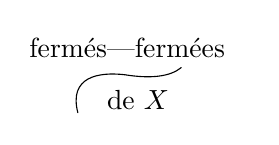
\begin{tikzpicture}[baseline=(opening.base),x=.013cm,y=-.013cm,line cap=round]
\path[use as bounding box] (-48,0) rectangle (170,87);
\node[anchor=base west,inner sep=0] at (-47,29) {\inserted{\unsure{fermés|fermées}}};
\node[anchor=base west,inner sep=0] (opening) at (29,80) {de $X$};
\draw (1,83) .. controls (-8,48) and (21,43) .. (47,46)
 .. controls (72,50) and (91,48) .. (102,39);
\end{tikzpicture}
(noté indiciellement), telles que l'on ait
% slanted
\reversemarginpar
\margin{$\nearrow$ On suppose de plus que pour \unsure{tte|toute|tt} comp. conn. $\unsure{\Sigma_i|\Sigma}$ de $X\setminus E_i$, on ait $\overline{\Sigma}_i\cap E_i\ne\varnothing$ i.e. $\overline{\Sigma}_i\ne\Sigma_i$ i.e. $\Sigma_i$ non fermé dans $X$ (ce qui est le cas si $X$ est connexe)}
\normalmarginpar
\[
 \forall i\in I,\quad \operatorname{Card}\pi_0(X\setminus\deleted{\Sigma}E_i)=2
 \tag*{(a)}
\]
\margin{\uline{NB} les comp. conn. $\Sigma_i^+,\Sigma_i^{\unsure{+|-|\ast}}$ de $X\setminus\Sigma_i$ sont ouvertes dans $X$}
\[
 \begin{aligned}
 &\forall(i,j)\in I\times I,\ i\ne j,\quad \deleted{\Sigma}E_j\ \text{est contenu dans l'une}\\
 &\text{des deux composantes connexes de }X\setminus\deleted{\Sigma}E_i.
 \end{aligned}
 \tag*{(b)}
\]

NB Cette condition (b) est vérifiée automatiquement les $\deleted{\Sigma}E_i$ $(i\in I)$ sont connexes, dès lors que les $E_i$ sont supposés disjoints mutuellement

On se propose d'étudier le ``découpage'' de $X$ par la famille $(E_i)$.

% RULE01: full-scan origin (501,996); long wavy underline and separate short run under 2.
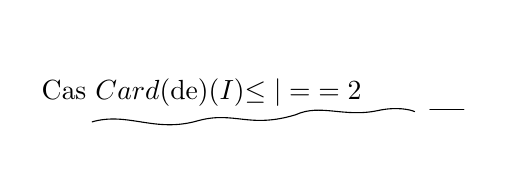
\begin{tikzpicture}[baseline=(case.base),x=.013cm,y=-.013cm,line cap=round]
\path[use as bounding box] (0,0) rectangle (443,117);
\node[anchor=base west,inner sep=0] (case) at (13,70)
 {Cas $\operatorname{Card}\deleted{\unsure{(\mathrm{de})}}(I)\deleted{\unsure{\leq|=}}=2$};
\draw (63,92) .. controls (98,82) and (124,103) .. (166,91)
 .. controls (202,81) and (216,99) .. (262,85)
 .. controls (286,74) and (309,88) .. (342,81)
 .. controls (360,77) and (374,80) .. (378,82);
\draw (393,80) -- (426,80);
\end{tikzpicture}

Soit $\Sigma_i^+$ la comp. conn. de $X\setminus E_i$ qui ne contient pas $E_j$ $(j\ne i)$, alors on a (si $I=\{1,2\}$)
% Drawing coordinates retain C's local map: full-scan approximately (x+24,y+1069).
% The lower-right contour is interrupted at observed bbox (394,1278,413,1308).
\figure{\begin{tikzpicture}[x=.013cm,y=-.013cm,line cap=round,line join=round]
\path[use as bounding box] (-10,-20) rectangle (535,300);
\draw (182,89) .. controls (226,-13) and (337,-39) .. (379,72)
 .. controls (405,143) and (409,181) .. (384,212);
\draw (376,226) .. controls (359,258) and (333,277) .. (303,281)
 .. controls (217,298) and (139,247) .. (161,158)
 .. controls (157,176) and (155,135) .. (182,89);
\draw[line width=.8pt] (181,89) .. controls (256,91) and (313,77) .. (382,86)
 (174,218) .. controls (240,224) and (317,212) .. (380,212);
\draw (44,9) .. controls (46,57) and (63,106) .. (32,108)
 .. controls (52,132) and (38,151) .. (46,195) -- (55,228);
\draw (41,109) .. controls (72,143) and (35,144) .. (48,193)
 .. controls (47,224) and (57,241) .. (39,252) .. controls (55,242) and (43,259) .. (49,282);
\draw (428,86) .. controls (439,93) and (409,141) .. (434,149)
 .. controls (420,158) and (436,251) .. (417,254);
% CANCEL01: glyph retained once; observed oblique crossing strokes replace a generic horizontal strike.
\node at (166,20) {\rlap{$\unsure{\Sigma_1^+|\Sigma_2^+}$}\phantom{$\deleted{\unsure{\Sigma_1^+|\Sigma_2^+}}$}};
\draw[line width=.65pt] (135,37) -- (185,-10);
\draw[gray,line width=.45pt] (155,7) -- (177,-12) -- (170,9);
\node at (139,90) {$E_1$}; \node at (149,220) {$E_2$};
\node at (429,32) {$\Sigma_1^+$};
\node at (492,160) {$\Sigma_1^{\deleted{\unsure{+}}\unsure{-}}$};
\node at (14,111) {$\Sigma_2^-$}; \node at (115,278) {$\Sigma_2^+$};
% MARK02: detached spot above the right label; full scan (528,1193,531,1197).
\node[inner sep=0] at (505,126) {\unsure{\begin{tikzpicture}[x=.013cm,y=-.013cm]
\path[use as bounding box] (0,0) rectangle (4,5);
\fill (0,0) .. controls (3,0) and (4,3) .. (2,4) .. controls (0,4) and (0,1) .. cycle;
\end{tikzpicture}}};
\end{tikzpicture}}
\[
 \Sigma_1^+\cap\Sigma_2^+=\varnothing
 \tag*{(1)}
\]
ce qui \deleted{résulte de}
\[
 \begin{aligned}
 &\begin{tikzpicture}[baseline=(inc.base),x=.013cm,y=-.013cm,line cap=round]
 \path[use as bounding box] (0,0) rectangle (329,79);
 \node[anchor=base west,inner sep=0] (inc) at (2,59)
 {\rlap{$\Sigma_1^-\supset\Sigma_2^+$}\phantom{$\deleted{\Sigma_1^-\supset\Sigma_2^+}$}};
 % CANCEL02: original full-scan origin (704,1388).
 \draw (2,54) .. controls (149,38) and (243,44) .. (325,37);
 % MARK03: two detached points above the relation, observed (859,1404,863,1411).
 \node[inner sep=0] at (157,19) {\unsure{\begin{tikzpicture}[x=.013cm,y=-.013cm]
 \path[use as bounding box] (0,0) rectangle (5,8);
 \fill (3,0) circle[radius=.8]; \fill (1,6) circle[radius=1];
 \end{tikzpicture}}};
 \end{tikzpicture}
 \qquad\text{équivaut à}\\
 &\deleted{\Sigma_2^-\supset\Sigma_1^+}\qquad \Sigma_1^+\subset\Sigma_2^-\cup E_2,\quad\text{et}
 \end{aligned}
\]
% CANCEL03: two distinct strokes, full-scan origin (202,1435).
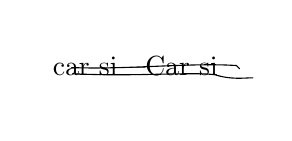
\begin{tikzpicture}[baseline=(carsi.base),x=.013cm,y=-.013cm,line cap=round]
\path[use as bounding box] (0,0) rectangle (231,83);
\node[anchor=base west,inner sep=0] (carsi) at (24,47)
 {\rlap{\unsure{car si|Car si}}\phantom{\deleted{\unsure{car si|Car si}}}};
\draw (43,39) .. controls (99,41) and (160,34) .. (204,37) -- (207,40);
\draw (44,45) .. controls (104,48) and (161,43) .. (183,46)
 .. controls (199,51) and (211,49) .. (220,49);
\end{tikzpicture}
\deleted{Si on avait} comme $\Sigma_1^+\cap E_2=\varnothing$, cela équivaut aussi à
\[
 \Sigma_1^+\subset\Sigma_2^-
 \tag*{(2)}
\]
% MARK04: independent right-side pair, full scan (1603,1778,1610,1786).
\margin{\unsure{\begin{tikzpicture}[x=.013cm,y=-.013cm]
\path[use as bounding box] (0,0) rectangle (9,10);
\fill (6,1) .. controls (8,0) and (9,2) .. (6,4) .. controls (4,4) and (4,2) .. cycle;
\fill (1,7) .. controls (3,6) and (5,7) .. (3,9) .. controls (1,9) and (0,8) .. cycle;
\end{tikzpicture}}}
\unsure{et} symétriquement, à
\[
 \Sigma_2^+\subset\Sigma_1^-
 \tag*{$(2')$}
\]

Comme
% MARK05: detached slant between the cancelled words and Sigma; source (510,2061,528,2076).
$\overset{\begin{smallmatrix}\text{\deleted{vois. ouvert}}\\
\text{\unsure{\begin{tikzpicture}[x=.013cm,y=-.013cm]
\path[use as bounding box] (0,0) rectangle (19,17);
\draw[line cap=round,line width=.7pt] (1,15) .. controls (8,6) and (12,3) .. (18,1);
\end{tikzpicture}}}
\end{smallmatrix}}{\Sigma_2^-}\supset E_1$,
\deleted{il contient les} \inserted{i.e. $\Sigma_2^-$ est un \uline{vois}. ouvert de $E_1$,} on \unsure{a}
% slanted; local note coordinates are full-scan coordinates minus (17,1962).
% GUIDE02 and GUIDE03 are separate observed curved strokes, without a supplied mathematical role.
\reversemarginpar
\margin{\figure{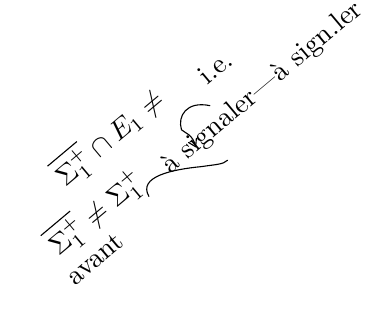
\begin{tikzpicture}[x=.009cm,y=-.009cm,line cap=round]
\path[use as bounding box] (0,0) rectangle (445,383);
\node[rotate=40,inner sep=0] at (114,154) {$\overline{\Sigma_1^+}\cap E_1\ne\varnothing$};
\node[rotate=40,inner sep=0] at (264,56) {i.e.};
\node[rotate=40,inner sep=0] at (95,260) {$\overline{\Sigma_1^+}\ne\Sigma_1^+$};
\node[rotate=40,inner sep=0] at (331,85) {\unsure{à signaler|à sign.ler}};
\node[rotate=40,inner sep=0] at (94,326) {avant};
% Approximate paths: GUIDE02 observed near (233,2071)-(274,2131).
\draw (257,110) .. controls (224,103) and (211,125) .. (217,144)
 .. controls (222,149) and (233,150) .. (237,168);
\draw (237,168) -- (227,162) (237,168) -- (238,156);
% GUIDE03 observed near (187,2149)-(300,2200).
\draw (171,238) .. controls (155,210) and (204,200) .. (245,196)
 .. controls (265,193) and (276,193) .. (282,187);
\end{tikzpicture}}}
\normalmarginpar
\[
 \Sigma_2^-\cap\Sigma_1^+\ne\varnothing
\]
Car
% RULE02: hooked short underline, observed full bbox (896,2226,1038,2245).
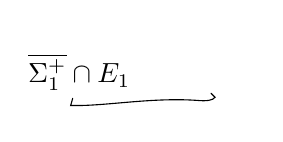
\begin{tikzpicture}[baseline=(carformula.base),x=.013cm,y=-.013cm,line cap=round]
\path[use as bounding box] (0,-54) rectangle (222,30);
\node[anchor=base west,inner sep=0] (carformula) at (0,0) {$\overline{\Sigma_1^+}\cap E_1$};
\draw (44,15) -- (42,22) .. controls (75,23) and (119,14) .. (165,17)
 .. controls (175,18) and (181,17) .. (183,14) -- (179,10);
\end{tikzpicture}
$\ne\varnothing$ (sinon
% GUIDE04: full-scan origin (1455,2104), original guide around (1460,2151)-(1604,2200).
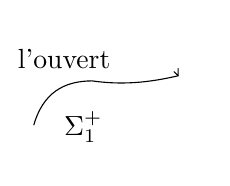
\begin{tikzpicture}[baseline=(sigmaopen.base),x=.013cm,y=-.013cm,line cap=round]
\path[use as bounding box] (0,0) rectangle (170,127);
\node[anchor=base west,inner sep=0] at (-10,40) {\inserted{l'ouvert}};
\node[anchor=base west,inner sep=0] (sigmaopen) at (35,105) {$\Sigma_1^+$};
\draw (6,95) .. controls (15,64) and (35,52) .. (63,52)
 .. controls (91,56) and (117,54) .. (147,47);
\draw (147,47) -- (143,43) (147,47) -- (147,40);
\end{tikzpicture}
serait \inserted{un} fermé dans $X$, \unsure{donc|puis}
% CANCEL04: same recovered group as C, with explicit oblique crossings over the initial symbol.
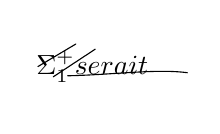
\begin{tikzpicture}[baseline=(lastcancel.base),x=.013cm,y=-.013cm,line cap=round]
\path[use as bounding box] (0,-26) rectangle (160,50);
\node[anchor=base west,inner sep=0] (lastcancel) at (8,20)
 {\rlap{$\unsure{\Sigma_1^+\text{ serait}}$}\phantom{$\deleted{\unsure{\Sigma_1^+\text{ serait}}}$}};
\draw (10,12) -- (47,-10); \draw (25,22) -- (66,-5);
\draw (39,21) .. controls (84,20) and (126,14) .. (156,18);
\end{tikzpicture}
$X$ serait disconnexe),
\endgroup
% archive sheet number: 14
